\section{触摸延时开关电路图}
上一节,我们了解了绘制电子电器元件的方法及电子元器件图块的制作方法。这一节中,我们将应用我们所做的电子元器件图块和CAD绘图技巧完成本章开始所展示的触摸延时开关电路图。
\subsection{绘制参考线}
为使绘制的电路图整齐美观,我们要先建立一个参考线图层,并用Xline绘制参考线,以便于电子元件定位。建立图层的方法请参看\ref{sec:falan}图层管理的相关内容,此处不再重复。

\noindent
命令: xline
指定点或 [水平(H)/垂直(V)/角度(A)/二等分(B)/偏移(O)]: 0,0
指定通过点:$ @1<0$
指定通过点: $@1<90$
指定通过点:

然后以30mm为间距对参考线进行偏移,形成参考线网格,具体过程在此不再重复,如图\ref{fig:cankaoxian}所示。

\noindent
\begin{figure}[htbp]
\centering
\begin{floatrow}
\ffigbox{\caption{参考线}\label{fig:cankaoxian}}{

\includegraphics[scale=0.4]{cankaoxian.png}
}
\ffigbox{\caption{块插入}\label{fig:kuaicaru}}{
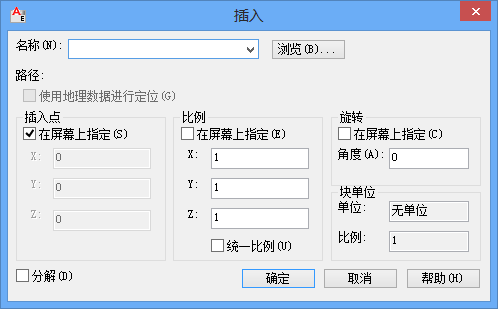
\includegraphics[scale=0.45]{kuaicaru.png}
}
\end{floatrow}
\end{figure}
\subsection{绘制电器元件}
参考线绘制完成后,我们就开始绘制电子元器件,其绘制方法主要是进行块插入操作,即加载相应的电子元器件图块,并将其放到相应的参考线上。

块的插入操作比较简单,当输入insert后好即出现图\ref{fig:kuaicaru}所示对话框,点击【浏览】按钮,找到相应的电子元器件文件并确定,实现元件块调入,接下来填写相应的参数,最后点击确定。

由于块插入操作是一致的,我们在此只以桥式电路元件为例进行演示,其它元件的绘制以此为参照即可,不在鳌述,最络结果如图\ref{fig:onlydianziyujian}所示。
\noindent
命令:INSERT\\
指定插入点或 [基点(B)/比例(S)/X/Y/Z/旋转(R)]:\\
命令: insert\\
指定插入点或 [基点(B)/比例(S)/X/Y/Z/旋转(R)]: r\\
指定旋转角度 $<0>$: 180\\
指定插入点或 [基点(B)/比例(S)/X/Y/Z/旋转(R)]:\\
命令: insert\\
指定插入点或 [基点(B)/比例(S)/X/Y/Z/旋转(R)]:\\
命令: INSERT\\
指定插入点或 [基点(B)/比例(S)/X/Y/Z/旋转(R)]: r\\
指定旋转角度 $<0>$: 180\\
指定插入点或 [基点(B)/比例(S)/X/Y/Z/旋转(R)]:\\
命令: insert\\
指定插入点或 [基点(B)/比例(S)/X/Y/Z/旋转(R)]:\\

\noindent
\begin{figure}
\centering
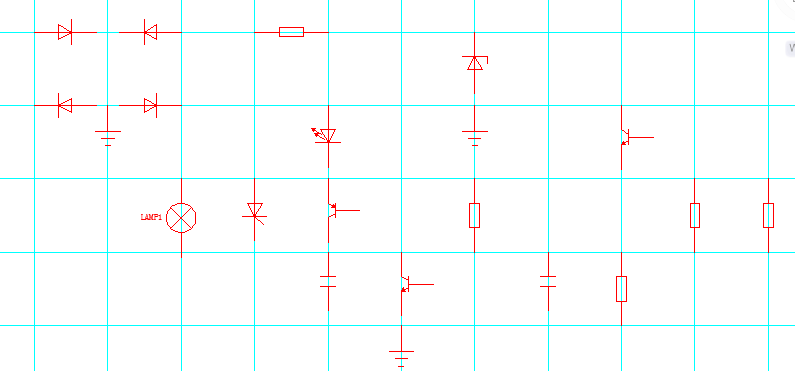
\includegraphics[scale=0.6]{onlydianjiyuanjian.png}
\caption{电路元件图}\label{fig:onlydianziyujian}
\end{figure}
\subsection{绘制线路}
最后,我们根据电路的特点,新建图层并绘水平或垂直连接线即可完成电路图,其过程与图形的绘相同因此就不在一一叙述了。最终结果如图\ref{fig:zhumodianlu}所示。

\zhishi{insert命令解析}
\endinput